\chapter{Вторая глава. Описание моделей}
\label{cha:ch_2}
\section{Модель раскрытия совместного преступления}
Модель раскрытия совместного преступления, предложенная Спенглером \cite{Spengler}, предполагает игру в развернутой форме для трех игроков с эндогенным характером формирования игровых историй.
Игра построена следующим образом. В игре учавствуют три игрока: клиент(C), чиновник(O) и инспектор(I). Игру начинает клиент. Клиент может подкупить чиновника с вероятностью $\gamma$ или нет с вероятностью $1 - \gamma$. Чиновник, в случае подкупа, может ответить взаимностью с вероятностью $\beta$ или нет с вероятностью $1 - \beta$. Взаимность определяется как акт возврата благосклонности за взятку, то есть возвращение некоторых привелегий (например, государственный контракт) клиенту. Коррупция, как взаимное взяточничество, может произойти только при совместных усилиях клиента и чиновника. Игра включает в себя четыре штрафа, один за подкуп $p_L$ и один для получения взаимности $q_L$ (штрафы клиента), а также один для принятия взятки и взаимности $q$ (штраф чиновника). Это позволяет использовать асимметричное распределение штрафов. Штрафы применяются с вероятностью инспектирования, которая представлена действием инспектора. Таким образом инспектор может провести проверку c вероятностью $\alpha$, либо не проводить с вероятностью $1 - \alpha$. При этом награда инспетора зависит факта инспектирования и наличия преступления. 
\par 
Для подкупа чиновника клиент тратит $b$ на взятку и получает выгоду от взаимности чиновника в размере $v$. Чиновник в случае подкупа получает взятку в размере $b$ , а неотвечая взяимностью получает $r$. Параметр $r$ играет роль нейтральной выплаты, для подкрепления непринятия взятки и может быть расценен как моральное удавлетворение от несовершения преступления. В случаях выявленного преступления клиент и чиновник должны выплатить соответствующие штрафы. 
Распределение выплат инспектору показано в таблице \ref{tbl:inspr1}.
\begin{table}[H]
	\centering
	\begin{tabular}[t]{|c|c|c|}
		\hline
		История игры & Провести проверку: $\alpha$ & Не проводить: $1-\alpha$ \\
		\hline
		Взаимная взятка: $\gamma \beta$ & $x + \Delta x$ & $x$ \\
		\hline
		Невзяимная взятка: $\gamma (1 - \beta$) &  $y + \Delta y$ & $y$ \\
		\hline
		Не было взятки: $(\gamma - 1)$ &  $z$ & $z + \Delta z$ \\
		\hline
	\end{tabular}
	\caption{\centering Схема распределения выплат инспектору}
	\label{tbl:inspr1}
\end{table}
\par
Предполагается, что проверка приводит к лучшим для инспектора результатам в случае (взаимного) взяточничества, чем в случае отсутствия взяточничества и наоборот: $0 <∆x, ∆y, ∆z$.
\par
Для клиента мы предполагаем, что взяточничество является прибыльным, если оно встречает взаимность, но не с проверкой, где $b$ - взятка, а $v$ - это выгода от взаимного обращения с клиентом. Это подразумевает, что $0 < b < v$ и $0 < p_L$, $p_H$ и $v - b - p_L - p_H <0$.
Для инспектора предполагется, что проверка является прибыльной, если по крайней мере один правонарушитель совершает правонарушения, но обходится дорого, если нет. Это подразумевает, что $x <0 <x + ∆x$ и $y <0 <y + ∆y$, но $z <0 <z + ∆z$. Эта настройка отражает интуицию, что успешный осмотр стоит того, поскольку он приводит к продвижению или аналогичным выгодам, в то время как безуспешная проверка просто стоит усилий. Сложность модели требует, чтобы мы сделали некоторые дополнительные предположения о выплатах инспектора. Мы предполагаем, что проверка взаимного взяточничества является более прибыльной, чем проверка простого взяточничества, и, аналогично, что не проверки взаимного взяточничество несет большую потерю, чем не проверка простого взяточничества из-за более высокой альтернативной стоимости неинспекции. Это подразумевает, что $0 <y + ∆y <x + ∆x$ и $x < y < 0$. Для чиновника мы предполагаем, что получение взятки является прибыльным, пока нет проверки, подразумевая, что $0 < r < b < q$.
\par
Последовательность выборов игроков и распределение выплат данной игры могут быть представлены в развернутой форме. Развернутая форма игры представлена на рисунке \ref{fig:figef1}.
\begin{figure}[H]
	\centering
	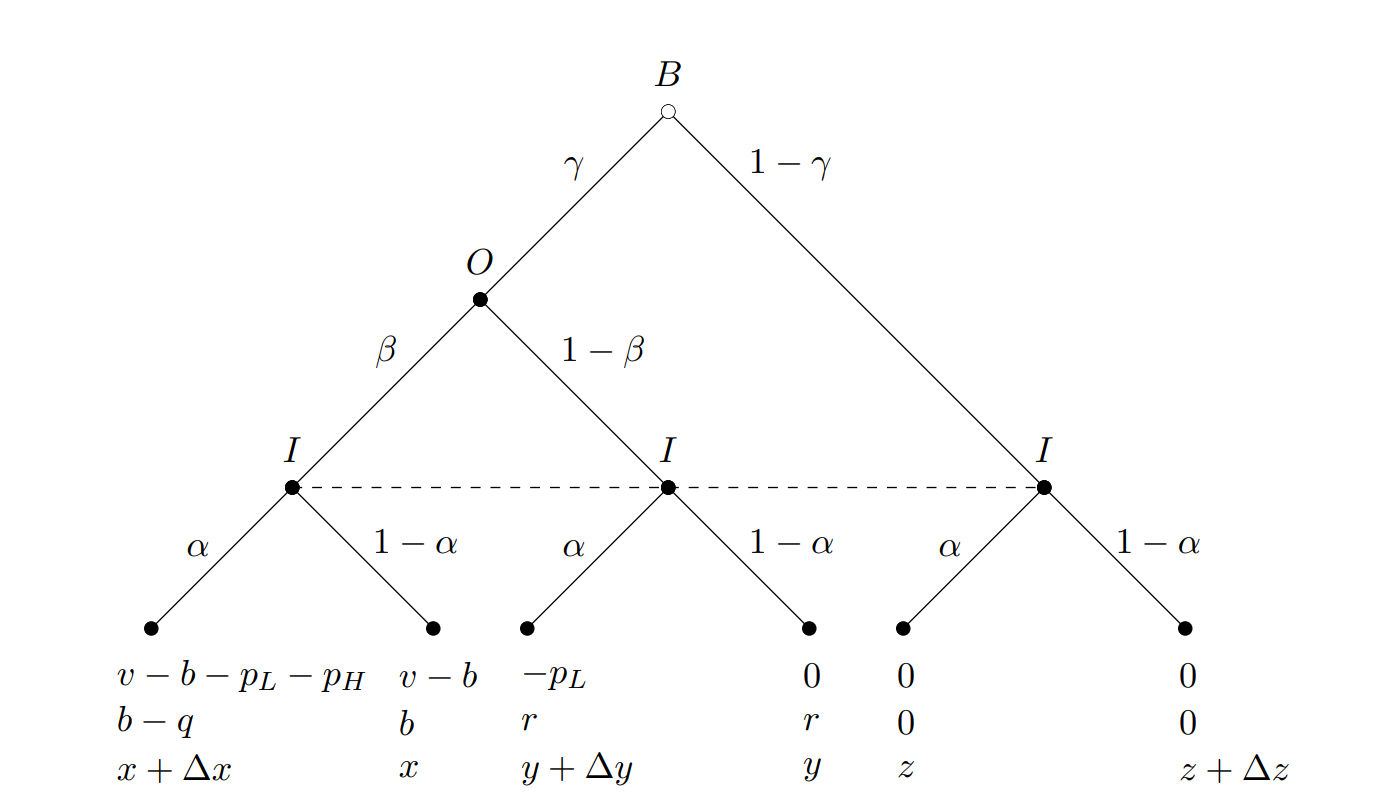
\includegraphics[width=0.9\linewidth]{inc/img/ef1}
	\caption{Развернутая форма игры}
	\label{fig:figef1}
\end{figure}
\par
Рассмотрим равновесие данной игры. Чтобы алгебраически выразить равновесие, для каждого игрока приравняем выплаты каждой стратегии. Используя выплаты на рисунке \ref{fig:figef1}, мы получаем уравнения (\ref{eq:2.1}), (\ref{eq:2.2}) и (\ref{eq:2.3}), связанные с выплатами клиента, чиновника и инспектора соответственно.
\begin{equation}\label{eq:2.1}
	\beta(v-b-\alpha(p_L + p_H)) + (1 - \beta)(-\alpha p_L)=0
\end{equation}
\begin{equation}\label{eq:2.2}
	\alpha(b-q) + (1-\alpha)b=\alpha r + (1-\alpha)r
\end{equation}
\begin{equation}\label{eq:2.3}
	\gamma \beta(x+\Delta x) + \gamma(1-\beta)(y+\Delta y) + (1 - \gamma)z = \gamma \beta x + \gamma(1-\beta)y + (1 - \gamma) (z + \Delta z)
\end{equation}
\par
Мы получаем следующие вероятности равновесия для $v$, $\beta$ и $\alpha$ из предыдущих уравнений:
\begin{equation}\label{eq:2.4}
	\beta = \frac{\alpha p_L}{v - b - \alpha p_H}
\end{equation}
\begin{equation}\label{eq:2.5}
	\alpha = \frac{b - r}{q}
\end{equation}
\begin{equation}\label{eq:2.6}
	\gamma = \frac{\Delta z}{\beta (\Delta x - \Delta y) + \Delta y + \Delta z}
\end{equation}
Дальнейшие преобразования (\ref{eq:2.4}-\ref{eq:2.6}) позволяют получить выражения $\beta$ и $\gamma$ заисящие от параметров:
\begin{equation}\label{eq:2.7}
	\alpha = \frac{(b - r)p_L}{(v - b)q - (b - r)p_H}
\end{equation}
\begin{equation}\label{eq:2.8}
	\gamma = \frac{((v-b)q - (b - r)p_H)\Delta z}{(b-r)p_L(\Delta x - \Delta y) + ((v-b)q-(b-r)p_H)(\Delta y + \Delta z)}
\end{equation}
\par
Относительно полученных значений можно отметить следующие предположения:
\begin{itemize}
	\item для клиента вероятность предложения взятки должна быть равна нулю, если вероятность принятия меньше вероятности принятия/возврата в уравнении (\ref{eq:2.4}) и равна одному в обратном случае;
	\item для чиновника вероятность принятия должна быть равна нулю, если вероятность проверки больше, чем вероятность проверки в уравнении (\ref{eq:2.5}) и равен одному в обратном случае;
	\item для инспектора вероятность проверки должна быть равна нулю, если вероятность предложения взятки меньше, чем вероятность предложения взятки в уравнении(\ref{eq:2.6}) и равна единице в обратном случае.
\end{itemize}
\par
Помимо приведенного выше примера, также рассматривается вариант данной игры, в котором не проводится проверка после отклонения взятки, а сразу выписывается штраф \cite{Spengler}. Но в силу того, что проверка коррупции часто инициируется заранее, то факт проверки часто не зависит от факта предложения взятки. Таким образом ограничемся только этим более обобщенным вариантом.
\section{Модель коррупции в иерархической структуре}
